\documentclass[a4paper,11pt]{article}

\usepackage[english]{babel}
\usepackage{float}
\usepackage{graphicx}
\usepackage{amsmath,amsthm}
\usepackage{gensymb}
\usepackage{amssymb}
\usepackage[margin=2.cm]{geometry}
\usepackage{pstricks-add}	%for geometric diagrams
\usepackage{chemfig}	%for structural formulae
\usepackage{tabularx}	%for better tables
\usepackage{booktabs}	%for better tables
\usepackage[makeroom]{cancel}	%for cancelling lines
\usepackage{hyperref}	%hyperlinks
\usepackage{mathrsfs}
\usepackage{mathtools}
\usepackage{epigraph}	%quotes
\usepackage{lastpage}
\usepackage{multicol}	%column environments
\usepackage{fancyhdr}	%headers
\usepackage[at]{easylist}	%easy lists
\usepackage{wasysym}
\usepackage{wrapfig}	%wrap figures in text
\usepackage{subfig}		%subfigures
\usepackage{tikz}

\allowdisplaybreaks
\newcommand\numberthis{\addtocounter{equation}{1}\tag{\theequation}}
\setlength{\epigraphwidth}{7.7cm}
\setlength{\tabcolsep}{10pt}

% bracket group shorthands
\newcommand{\abs}[1]{\left|#1\right|}
\newcommand{\set}[1]{\left\{#1\right\}}

% common sets
\newcommand{\R}{\mathbb{R}}
\newcommand{\Cmplx}{\mathbb{C}}
\newcommand{\Q}{\mathbb{Q}}
\newcommand{\Z}{\mathbb{Z}}
\newcommand{\N}{\mathbb{N}}

% derivative shorthands
\newcommand{\diff}[2]{\frac{\mathrm{d}#1}{\mathrm{d}#2}}
\newcommand{\pdiff}[2]{\frac{\partial #1}{\partial #2}}
\newcommand{\ndiff}[3]{\frac{\mathrm{d}^{#3}#1}{\mathrm{d}#2^{#3}}}
\newcommand{\npdiff}[3]{\frac{\partial^{#3} #1}{\partial #2^{#3}}}

% theorem environments
\newtheorem*{definition*}{Definition}
\newtheorem*{lemma*}{Lemma}
\newtheorem{theorem}{Theorem}
\newtheorem*{theorem*}{Theorem}
\newtheorem*{corollary*}{Corollary}
\newtheorem{example}{Example}
\newtheorem*{remark}{Remark}

\DeclareMathOperator{\bdy}{Bdy}
\DeclareMathOperator{\interior}{Int}

% header
\pagestyle{fancy}
\lhead{An Introduction to Differential Calculus}
\rhead{Year 11 2018}

\title{An Introduction to Differential Calculus}
\date{\today}
\author{Daniel Czapski}

\begin{document}
	\maketitle
	\begin{abstract}
		This is a summary of the fundamentals of the calculus topic as studied in year 11. The motivation for the study of calculus is inherently physical. Calculus is an incredibly powerful tool that sees extensive application in almost all areas of physical life, from determining the flight paths of projectiles and planets to modelling the spread of disease, the growth of human population or the movement of oceans.  At its heart, we are attempting to study \textbf{rates of change}.
	\end{abstract}
	\tableofcontents
	\vfill
	%\begin{figure}[H]
%		\centering
%		
\includegraphics[width=0.4\textwidth]{t100}
%	\end{figure}
	\vfill
	\pagebreak
	%\section*{Differential Calculus -- Cheat Sheet -- Year 11 2018}
	
	\section{Definition}
	Remember the gradient.
	
	\begin{center}
		\begin{tikzpicture}[domain=-2.5:2.5,scale=1.34]
	\draw[->] (0,-2.5) -- (0,2.5) node[right]{$y$};
	\draw[->] (-2.5,0) -- (2.5,0) node[right]{$x$};
	\draw[domain=-2.5:1.25] plot (\x,1.2*\x+1);
	\node [right] at (0.5,1) {$y=\frac{6}{5}x+1$};
	\end{tikzpicture}
	\end{center}
	The gradient is the \textbf{rate of change of $y$ with respect to $x$}. In other words, it tells us how much $y$ changes when you change $x$ by one. Given two points on a line, $(x_1,y_1)$ and $(x_2,y_2)$, we can calculate the gradient:
	\begin{align*}
	m = \frac{y_2-y_1}{x_2-x_1} = \frac{\Delta y}{\Delta x}
	\end{align*}
	where we say that $\Delta y = y_2-y_1$ and $\Delta x=x_2-x_1$. Crucially, we need \textbf{two} points on a line to define a gradient.\\
	
	\noindent Now, consider a curve which is \textbf{not} a straight line.
	\begin{center}
		\begin{tikzpicture}[domain=-0.5:2.5,scale=1.68]
		\draw[->] (0,-0.5) -- (0,2.5) node[right]{$y$};
		\draw[->] (-2.5,0) -- (2.5,0) node[right]{$x$};
		\draw[domain=-1.58:1.58,samples=50] plot (\x,\x*\x);
		\node [right] at (1.25,1) {$y=x^2$};
		\end{tikzpicture}
	\end{center}

	This is just a parabola. We know the equation of the curve, and have an intuitive understanding of its behaviour -- when we change $x$ to $x+1$, the $y$ value increases from $x^2$ to $(x+1)^2$. But how can we quantify this? What if our curve isn't something simple, like a parabola, but is something a bit more messed up, like $f(x) = \sin\left(\frac{1-\sqrt{5x^{7/3}}}{12}\right)-x^3$? We need something more general.\\
	
	\noindent The easiest place to start is to consider \textbf{tangent lines}. 
	
	\begin{center}
		\begin{tikzpicture}[domain=-0.5:2.5,scale=1.68]
		\draw[->] (0,-0.5) -- (0,2.5) node[right]{$y$};
		\draw[->] (-2.5,0) -- (2.5,0) node[right]{$x$};
		\draw[domain=-1.58:1.58,blue,thick,samples=50] plot (\x,\x*\x);
		\draw[domain=0.25:1.75,red,dashed,thick] plot (\x,2*\x-1);
		\draw[fill=black] (1,1) circle [radius=0.04];
		
		\node [left] at (-1.25,1) {$y=f(x)$};
		\node [right] at (1,1) {$(x,f(x))$};
		\end{tikzpicture}
	\end{center}
	
	If we take the gradient of a tangent line, we get a measure of the slope \textbf{at a point}, and we're done. However, we run into a problem. We need \textbf{two} points to calculate a gradient. Here, we only have \textbf{one}! We remedy this problem by first considering a \textbf{secant}. We take the point we're interested in, say $(x,f(x))$, and another point \textbf{at a small distance $h$ away} -- say $(x+h,f(x+h))$.
	
	\begin{center}
		\begin{tikzpicture}[domain=-0.5:2.5,scale=3]
		\draw[->] (0,-0.5) -- (0,2.5) node[right]{$y$};
		\draw[->] (-2.5,0) -- (2.5,0) node[right]{$x$};
		\draw[domain=-1.58:1.58,blue,thick,samples=50] plot (\x,\x*\x);
		\draw[dashed, domain=0.25:1.75,red,thick] plot (\x,2*\x-1);
		\draw[domain=0.4:1.6,green,thick] plot (\x,2.5*\x-1.5);
		\draw[fill=black] (1,1) circle [radius=0.02];
		\draw[fill=black] (1.5,2.25) circle [radius=0.02];
		\draw[dashed] (1,1) -- (1,-0.05) node[below] {$x$};
		\draw[dashed] (1,1) -- (-0.05,1) node[left] {$f(x)$};
		\draw[dashed] (1.5,2.25) -- (1.5,-0.02) node[below] {$x+h$};
		\draw[dashed] (1.5,2.25) -- (-0.05,2.25) node[left] {$f(x+h)$};
		
		\node [left] at (-1.25,1) {$y=f(x)$};
		%\node [above left] at (1,1) {$(x,f(x))$};
		%\node [left] at (1.5,2.25) {$(x+h,f(x+h))$};
		\end{tikzpicture}
	\end{center}

	It's not quite a tangent, but it's pretty close. So, if we calculate the gradient of this secant using the formula we're familiar with, it should be pretty close to that of our tangent:
	\begin{align*}
	m_s = \frac{f(x+h)-f(x)}{h} = \frac{\Delta y}{\Delta x}.
	\end{align*}
	But we can do better. If we take our second point and \textbf{move it closer to the first}
	
	\begin{center}
		\begin{tikzpicture}[domain=-0.5:2.5,scale=3]
		\draw[->] (0,-0.5) -- (0,2.5) node[right]{$y$};
		\draw[->] (-2.5,0) -- (2.5,0) node[right]{$x$};
		\draw[domain=-1.58:1.58,blue,thick,samples=50] plot (\x,\x*\x);
		\draw[dashed, domain=0.25:1.75,red,thick] plot (\x,2*\x-1);
		\draw[domain=0.318:1.68,green,thick] plot (\x,2.2*\x-1.2);
		\draw[fill=black] (1,1) circle [radius=0.02];
		\draw[fill=black] (1.2,1.44) circle [radius=0.02];
		\draw[dashed] (1,1) -- (1,-0.05) node[below] {$x$};
		\draw[dashed] (1,1) -- (-0.05,1) node[left] {$f(x)$};
		\draw[dashed] (1.2,1.44) -- (1.2,-0.02) node[below right] {$x+h$};
		\draw[dashed] (1.2,1.44) -- (-0.05,1.44) node[left] {$f(x+h)$};
		
		\node [left] at (-1.25,1) {$y=f(x)$};
		%\node [right] at (1,1) {$(x,f(x))$};
		%\node [left] at (1.2,1.44) {$(x+h,f(x+h))$};
		\end{tikzpicture}
	\end{center}
	then we get even closer. \textbf{Moving the point closer is the same as making $h$ smaller}, because $h$ is the distance between the two $x$ values. So, we see that making $h$ smaller and smaller gives us better and better approximations to the gradient of the tangent. We can't make $h$ 0 directly; otherwise we would be dividing by zero, which is problematic. However, what we can do is consider what happens when $h$ gets ``very, very close'' to zero -- in other words, \textbf{take the limit}. As $h$ gets very close to zero, the gradient of the secant gets very close to the gradient of the tangent (hopefully the above argument somewhat convinces you of this fact). So,
	\begin{align*}
	m_T = \lim\limits_{h\to 0}m_s = \lim\limits_{h\to 0}\frac{f(x+h)-f(x)}{h} = \lim\limits_{h\to 0}\frac{\Delta y}{\Delta x}.
	\end{align*}
	Or, we write
	\begin{align*}
	m_T = \diff{y}{x} = \lim\limits_{h\to 0}\frac{f(x+h)-f(x)}{h}.
	\end{align*}
	This motivates the following definition.
	\begin{definition*}[Differentiation and the derivative]
		Consider a real-valued function $f$. Then, the \textbf{derivative}, denoted by $f'$, is given by 
		\begin{align*}
		f'(x) = \lim\limits_{h\to 0}\frac{f(x+h)-f(x)}{h}
		\end{align*}
		where this limit exists. If the derivative exists at some $x$, we say the function is \textbf{differentiable at $x$}. The process of finding the derivative is called \textbf{differentiation}. If the derivative of a function exists all all points in its domain, then we call it \textbf{differentiable everywhere}, or, simply \textbf{differentiable}.
	\end{definition*}

	\noindent In the preliminary and HSC courses, the process of finding the derivative using this formula is called \textbf{differentiation from/by first principles}.

	\begin{remark}
	\normalfont{It is interesting to note that differentiability at a point also implies continuity at a point -- i.e. differentiable functions are necessarily continuous. However, the converse is not true! Can you think of an example of a continuous function which has points where it is not differentiable? What about a function which is continuous everywhere, but differentiable nowhere?}
	\end{remark}
	
	\pagebreak
	\subsection*{Notation}
	We can denote the derivative in a number of ways, depending on how the question is presented to us. If we are given a function in the form $f(x)$, then we can write
	$$
	f'(x) =  \diff{f(x)}{x}
	$$
	equivalently. I prefer the first option, as it's more space efficient.\\
	
	\noindent If we are given an equation of the form $y=\cdots$, then we can write
	$$
	y' = \diff{y}{x}.
	$$
	If you see something like 
	$$
	\diff{}{x}\left(\cdots\cdots\right)
	$$
	then this means ``differentiate what's inside the brackets''\footnote{Technically, $\diff{}{x}$ is called an ``operator'', and it ``operates'' on whatever it touches. The operation is differentiation.}. Remember, \textbf{this is not a fraction!} It has nice properties which allow you to perform operations like a fraction, but it isn't one!
	
	\section{Finding Derivatives}
	You can do a couple of simple examples of finding derivatives from first principles, such as $x,1/\sqrt{x},x^2$ and the like.
	
	\begin{example}\normalfont
		Find the derivative of the function such that $f(x)=x^2$, from first principles.
		\begin{align*}
		f'(x) &= \lim\limits_{h\to 0}\frac{f(x+h)-f(x)}{h}\\
		&= \lim\limits_{h\to 0}\frac{(x+h)^2-x^2}{h}\\
		&= \lim\limits_{h\to 0}\frac{x^2+2xh+h^2-x^2}{h}\\
		&= \lim\limits_{h\to 0}\frac{2xh+h^2}{h}\\
		&= \lim\limits_{h\to 0}2x+h\\
		&= 2x.
		\end{align*}
	\end{example}
	
	However, it quickly becomes quite clear that using the definition is complicated and can be extremely tedious. It does not lend itself well to direct calculation. As such, we have a few \textbf{differentiation rules} which drastically simplify the process of finding derivatives.
	
	%\pagebreak
	
	\begin{theorem*}[Arithmetic properties of differentiation]
		Suppose $f$ and $g$ are differentiable, real-valued functions and $a\in\R$ ($a$ is some real number). Then,
		\begin{align*}
		\diff{}{x}\left(f(x)+g(x)\right) = \diff{}{x}f(x)+\diff{}{x}g(x)
		\end{align*}
		and 
		\begin{align*}
		\diff{}{x}\left(af(x)\right) = a\diff{}{x}f(x).
		\end{align*}
		In other words, \textbf{the derivative of a sum is the sum of the derivatives} and \textbf{you can pull constant factors out of derivatives}.
	\end{theorem*}

	\noindent However, unfortunately, 
		\begin{align*}
		\diff{}{x}\left(f(x)\times g(x)\right)\neq\diff{}{x}f(x)\times\diff{}{x}g(x)
		\end{align*}
		and
		\begin{align*}
		\diff{}{x}\left(\frac{f(x)}{g(x)}\right)\neq\frac{\diff{}{x}f(x)}{\diff{}{x}g(x)}.
		\end{align*}
	We need another theorem for that. \textbf{Remember this; forgetting it is a common mistake!}\\

	\noindent So, we can differentiate sum and multiples of functions that we could already differentiate on their own. Now that we have the basic machinery down-pat, we can think about trying to extend this idea to as many functions as we can.
	
	\subsection{Important differentiation rules}
	\begin{theorem*}[Power rule]
		Suppose $n\in\R$. Then,
		$$
		\diff{}{x}\left(x^n\right) = nx^{n-1}.
		$$
	\end{theorem*}
	This, combined with the arithmetic properties, allows us to differentiate polynomials and all real powers of $x$.
	\begin{theorem*}[Chain rule]
		Suppose $y$ is a function of $u$, and $u$ is a function of $x$. Then,
		$$
		\diff{y}{x} = \diff{y}{u}\times\diff{u}{x}.
		$$
	\end{theorem*}
	This essentially means that we can treat derivatives like fractions in some circumstances, and allows us to find the derivatives of functions like $(2x-3)^5$ without having to spend twenty minutes expanding it.
	\begin{theorem*}[Product Rule]
		Suppose $y = uv$, where $u$ and $v$ are functions of $x$. Then,
		\begin{align*}
		\diff{y}{x} &= u'v+uv'\\
		&= v\times\diff{u}{x}+u\times\diff{v}{x}.
		\end{align*}
	\end{theorem*}
	This allows us to differentiate products of functions we can differentiate individually. Finally,
	\begin{theorem*}[Quotient Rule]
		Suppose $y=\frac{u}{v}$ where $u$ and $v$ are functions of $x$, and $v(x)\neq 0$. Then,
		$$
		\diff{y}{x} = \frac{vu'-uv'}{v^2}.
		$$
	\end{theorem*}
	This allows us to differentiate fractions.\\
	
	
	\begin{remark}
		\normalfont
		There are a couple of important points to note.
		\begin{easylist}[itemize]
			@ It is imperative that you remember these rules and how to use them! \textbf{Once you learn them, they will be assumed knowledge for the rest of your course.}
			@ \textbf{The derivative evaluated at a point $x_0$ is the gradient of the tangent to the curve at the point $x_0$.} Finding the gradient of the tangent to a curve is a reason we developed this machinery in the first place! This is equivalent to the (instantaneous) rate of change of the function with respect to $x$ -- i.e. how much the function is changing with respect to $x$ at that particular point\footnote{If this last little point seems elusive, don't worry -- it is! How can we talk about a rate of change ``at a point'' when we're talking about changing $x$, which changes the point? The (somewhat) answer is that we consider ``infinitesimal'' changes; we change $x$ by such a small amount that it's basically negligible (sort of). Don't worry -- this is a subtle point and is much less important than the overarching ideas: gradients of tangents and the definition.}.
		\end{easylist}
	\end{remark}

	\noindent We also have a couple of handy facts which follow from the definition that are good to remember.
	\begin{corollary*}
		Suppose $C\in\R$ is a constant. Then,
		\begin{align*}
		\diff{}{x}\left(C\right) &= 0 && \diff{}{x}\left(x\right) = 1.
		\end{align*}
		In other words, \textbf{the derivative of a constant is zero}.
	\end{corollary*}
	\noindent With all of these rules combined, we can now differentiate functions involving sums, multiples and products of powers of $x$.
	
	\section{Applications}
	Differentiation allows us to analyse the behaviour of functions in new ways. In particular, there are a few major applications of differentiation that we study in the HSC course:
	\vspace{0.15cm}
	\begin{easylist}[itemize]
		\ListProperties(Margin1=1cm)
		@ Finding equations of tangents and normals
		@ Identifying and classifying stationary points
		@ Examining concavity
	\end{easylist}
	\subsection{Tangents and Normals}
	Recall that the formalism of calculus has been developed with the aim of \textbf{finding gradients of tangents}. Given a function and a point, we can use differentiation to find the gradient of the tangent and then, using facts about linear functions, find the equations of tangents and normals.\\
	
	\noindent Given an equation and an $x$ value, the general method is as follows.
	\vspace{0.15cm}
	\begin{easylist}[enumerate]
	\ListProperties(Numbers1=a,Numbers2=r,Progressive=1cm,Margin1=1cm)
	@ Find the corresponding $y$ value using the given equation.
	@ Differentiate the function.
	@ To find the gradient of the tangent, evaluate the derivative at the $x$ value of the given point. 
	@@ To find the gradient of the normal, use the fact that $m_Tm_N=-1$.
	@ To find the equation of the line, use the point-gradient formula.
	\end{easylist}
\vspace{0.15cm}
	\noindent We illustrate with an example.
	
	\begin{example}
		Consider the function $y=x^2+x-2$. Find the equations of the tangent and normal at $x=2$.\\\\
		\normalfont{To begin, we find the $y$ coordinate of the point in question,
		\begin{align*}
		y = 2^2+2-2 = 4
		\end{align*}
		so our point is $(2,4)$\\\\
		To find the equation of the tangent and normal, we first need the gradient of the tangent. Thus, we need to differentiate our function. We have
		\begin{align*}
			y' &= \diff{}{x}\left(x^2+x-2\right)\\
			&= \diff{}{x}\left(x^2\right)+\diff{}{x}\left(x\right)-\diff{}{x}\left(2\right)\\
			&= 2x+1-0\\
			&= 2x+1
		\end{align*}
		through applying the arithmetic properties of differentiation and the power rule\footnote{You can omit intermediate steps, such as the second and third lines. It's good to write it all out a couple of times, but are not necessary once you understand the idea.}. The gradient of the tangent at $x=2$ is the derivative evaluated at $x=2$. So, 
		\begin{align*}
		m_T = 2(2)+1 = 5.
		\end{align*}
		Recall that the normal is the line \textbf{perpendicular to the tangent}, so, using the fact that $m_Tm_N = -1$, we can find the gradient of the normal
		\begin{align*}
		m_Tm_N&=-1\\
		\implies 5m_N&=-1\\
		\implies m_N &= -\frac{1}{5}.
		\end{align*}
		Now that we have gradients and a point, we can use the point-gradient formula from the linear functions topic to find the equations. We find,
		\begin{align*}
		y-4 = 5(x-2) && y-4 = -\frac{1}{5}(x-2)\\
		y-4 = 5x-10 && y-4=-\frac{1}{5}x+\frac{2}{5}\\
		y = 5x-6 && y = -\frac{1}{5}x+\frac{22}{5}
		\end{align*}
		for the tangent and normal respectively.\\\\
		We can plot this: the function is plotted in black, the tangent in red and normal in blue.
		
		\begin{center}
		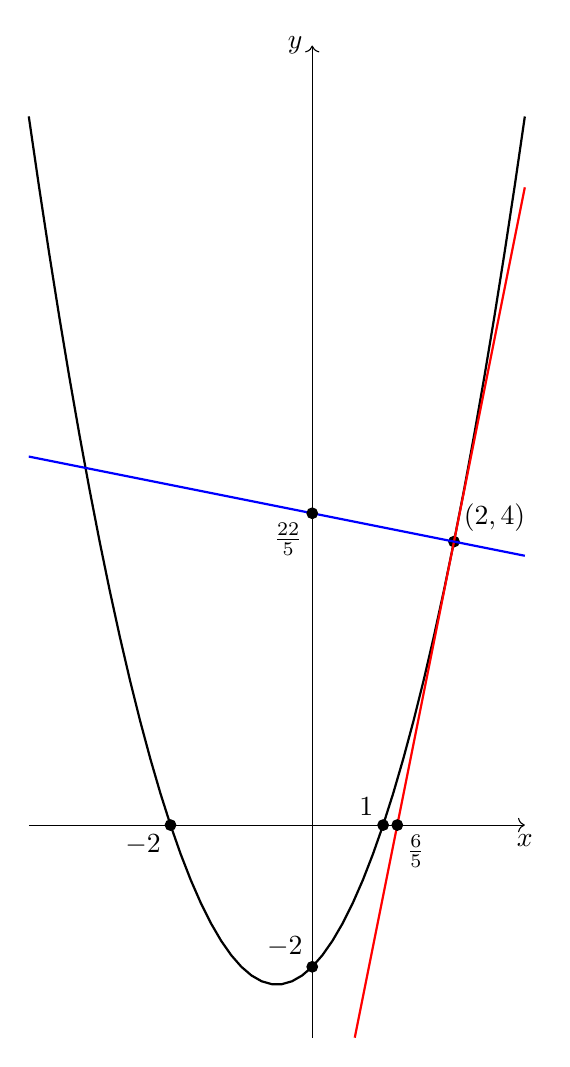
\begin{tikzpicture}[domain=-4:3,scale=0.9]
		\draw[->] (0,-3) -- (0,11) node[left] {$y$};
		\draw[->] (-4,0) -- (3,0) node[below] {$x$};
		\draw[thick,samples=50] plot (\x,\x*\x+\x-2);
		\draw[fill=black] (2,4) circle [radius=0.075] node[above right] {$(2,4)$};
		\draw[domain=0.6:3,thick,red] plot (\x,5*\x-6);
		\draw[domain=-4:3,thick,blue] plot (\x,-0.2*\x+4.4);
		\draw[fill=black] (0,4.4) circle [radius=0.075] node[below left] {$\frac{22}{5}$};
		\draw[fill=black] (1.2,0) circle [radius=0.075] node[below right] {$\frac{6}{5}$};
		\draw[fill=black] (1,0) circle [radius=0.075] node[above left] {$1$};
		\draw[fill=black] (-2,0) circle [radius=0.075] node[below left] {$-2$};
		\draw[fill=black] (0,-2) circle [radius=0.075] node[above left] {$-2$};
		\end{tikzpicture}
		\end{center}
	}
	\end{example}

	\subsection{Stationary Points}
	In terms of motion, if an object is ``stationary'', then it is not moving. In other words, the rate of change of its position with respect to time (i.e. its speed!) is zero. We can apply the same idea to quantities more generally by invoking calculus; specifically, \textbf{interpreting the derivative as a rate of change}. Hence, we write the following definition.
	
	\begin{definition*}[Stationary points]
		Consider a differentiable function $f$ and $x_0\in\R$. A \textbf{stationary point} is a point $(x_0,f(x_0))$ on the curve such that $f'(x_0)=0$. That is, \textbf{a stationary point is a point on a curve where the derivative is zero}.
	\end{definition*}
	\noindent If we go back to the idea that the derivative at $x_0$ is also the gradient of the tangent at $x_0$, then the above definition is equivalent to saying that \textbf{a stationary point is a point where the tangent is horizontal}.\\
	
	\noindent Thus, \textbf{to find stationary points}, we need simply find those points where the derivative is zero. That is, \textbf{we solve the equation $f'(x)=0$}.
	
	\begin{example}\normalfont
		Find all stationary points on the curve $y=x^3-6x^2-36x+10$.\\\\
		\normalfont{To begin, we need to differentiate. We have
			\begin{align*}
				y' &= \diff{}{x}\left(x^3-6x^2-36x+10\right)\\
				&= 3x^2-12x-36
			\end{align*}
			where we have omitted the intermediate steps. To find stationary points, we need to solve $y'=0$. That is,
			\begin{align*}
				3x^2-12x-36 &= 0\\
				3\left(x^2-4x-12\right) &= 0\\
				3(x-6)(x+2) &= 0\\
				\implies x &= -2,6.
			\end{align*}
			\textbf{We must also find the corresponding $y$-values.} At $x=-2$,
			$$
			y = (-2)^3-6(-2)^2-36(-2)+10 = 50
			$$
			and at $x=6$,
			$$
			y = 6^3-6\times6^2-36(6)+10 = -206.
			$$
			So, there are stationary points at $(-2,50)$ and $(6,-206)$.
		}
	\end{example}

	\subsection*{Classifying stationary points}
	We can divide stationary points into two main categories: \textbf{turning points} and \textbf{horizontal points of inflexion}. They are characterised by the \textbf{behaviour of the derivative on either side of the stationary point}. We can also split turning points up into \textbf{local maxima and minima}. In particular,
	\vspace{0.15cm}
	\begin{easylist}[itemize]
		\ListProperties(Margin1=1cm,Progressive=1cm)
		@ Turning points: the derivatives on either side have \textbf{different} signs.
		@@ Local maximum: \textbf{positive on the left, negative on the right}
		@@ Local minimum: \textbf{negative on the left, positive on the right}
		@ Horizontal points of inflexion: the derivatives on either side have \textbf{the same} sign.
	\end{easylist}
\vspace{0.15cm}
Working out what sort of stationary point is present is called \textbf{determining the nature} of the stationary point.

\begin{figure}[H]
	\centering
	\subfloat[Local maximum]{
		\begin{tikzpicture}[domain=-2:2,scale=2]
		\draw[->] (0,-1) -- (0,2) node[left] {$y$};
		\draw[->] (-2,0) -- (2,0) node[below] {$x$};
		\draw[domain=-1.34:1.74] plot (\x,-\x*\x+0.4*\x+1.34);
		\end{tikzpicture}
	}
	\subfloat[Local minimum]{
	\begin{tikzpicture}[domain=-2:2,scale=2]
		\draw[->] (0,-1) -- (0,2) node[left] {$y$};
		\draw[->] (-2,0) -- (2,0) node[below] {$x$};
		\draw[domain=-1.74:1.34] plot (\x,\x*\x+0.4*\x-0.34);
	\end{tikzpicture}
	}\\
	\subfloat[Horizontal point of inflexion]{
	\begin{tikzpicture}[domain=-2:2,scale=2]
		\draw[->] (0,-1) -- (0,2) node[left] {$y$};
		\draw[->] (-2,0) -- (2,0) node[below] {$x$};
		\draw[domain=-0.76:1.51] plot (\x,\x*\x*\x-0.9*\x*\x+0.27*\x+0.173);
	\end{tikzpicture}
	}
\end{figure}
\textbf{To determine the nature of a stationary point, check the sign of the derivative at points on either side of the stationary point}.

\begin{remark}\normalfont
	Be careful when choosing points! It is imperative that one chooses points that:
	\vspace{0.15cm}
	\begin{easylist}[itemize]
		\ListProperties(Margin1=1cm,Progressive=1cm)
		@ Have a well-defined value of the derivative;
		@ Are not other stationary points; and
		@ Do not have other stationary points between the chosen point and the stationary point being tested.
	\end{easylist}
\vspace{0.15cm}
\noindent Numbers like $\pm1$, $0$ and other integers are the easiest to use as they are usually easy to substitute into equations, but you can use whatever points you want, as long as they follow the above rules.
\end{remark}

\noindent The general method is as follows.
\vspace{0.15cm}
\begin{easylist}[enumerate]
	\ListProperties(Numbers1=a,Numbers2=r,Progressive=1cm,Margin1=1cm)
	@ Differentiate the function.
	@ Find the $x$-values of the stationary points.
	@ Find corresponding $y$-values.
	@ For each stationary point, choose a point on either side and test the value of the derivative at those points. Write these three points and the values of the derivatives at each in a table. Use this to determine the nature of the stationary point as per the rules prior.
\end{easylist}
\vspace{0.15cm}

\noindent We illustrate with another example. 
\pagebreak

\begin{example}\normalfont
	Find the coordinates and determine the nature of all stationary points on the curve $y=x^5-\frac{5}{4}x^4-\frac{10}{3}x^3$.\\\\
	First, we need to differentiate:
	\begin{align*}
		y' = 5x^4-5x^3-10x^2.
	\end{align*}
	To find stationary points, solve $y'=0$.
	\begin{align*}
		5x^4-5x^3-10x^2 &= 0\\
		5x^2\left(x^2-x-2\right) &= 0\\
		5x^2(x-2)(x+1) &= 0\\
		\implies x &= -1,0,2.
	\end{align*}
	So, there are stationary points at $x=-1,0$ and $1$. We need to find the corresponding $y$ values by substituting these $x$-values into the original equation. At $x=-1$, $y=-1-\frac{5}{4}+\frac{10}{3}= \frac{13}{12}$. At $x=0$, $y=0$. At $x=2$, $y=2^5-\frac{5}{4}\times2^4-\frac{10}{3}\times2^3= -\frac{44}{3}$.\\\\
	So, we have three stationary points at $(-1,\frac{13}{12})$, $(0,0)$ and $(2,-\frac{44}{3})$. To determine their nature, we need to test the value of the derivative at points on either side of each stationary point. A table is often the easiest and clearest way to present this information.\\\\
	For $(-1,\frac{13}{12})$, 
	{\renewcommand{\arraystretch}{1.5}%
	\begin{table}[H]\centering
		\begin{tabular}{c|c|c|c}
			$x$  &   $-2$    & $-1$ &  $-\frac{1}{2}$  \\ \hline
			$y'$ &   $80$    & $0$  & $-\frac{25}{16}$ \\
			 ~   & $\diagup$ & ---  &   $\diagdown$
		\end{tabular}
	\end{table}}
	The derivative is positive on the left and negative on the right, so we have a \textbf{local maximum at $(-1,\frac{13}{12})$.} Note that we cannot use 0, as we have a stationary point at $x=0$; we have to choose a point between $-1$ and $0$.\\\\
	For $(0,0)$, 
	{\renewcommand{\arraystretch}{1.5}%
		\begin{table}[H]\centering
			\begin{tabular}{c|c|c|c}
				$x$  &  $-\frac{1}{2}$  & $0$ &  $\frac{1}{2}$   \\ \hline
				$y'$ & $-\frac{25}{16}$ & $0$ & $-\frac{45}{16}$ \\
				 ~   &   $\diagdown$    & --- &   $\diagdown$
			\end{tabular}
	\end{table}}
	The derivative is negative on both the left and right, so we have a \textbf{horizontal point of inflexion at $(0,0)$.} Note that we cannot use $-1$, as we have a stationary point at $x=-1$; we have to choose a point between $-1$ and $0$.\\\\
	For $(2,-\frac{44}{3})$, 
	{\renewcommand{\arraystretch}{1.5}%
		\begin{table}[H]\centering
			\begin{tabular}{c|c|c|c}
				$x$  &  $\frac{1}{2}$   & $2$ &    $3$    \\ \hline
				$y'$ & $-\frac{45}{16}$ & $0$ &   $180$   \\
				 ~   &   $\diagdown$    & --- & $\diagup$
			\end{tabular}
	\end{table}}
	The derivative is negative on the left and positive on the right, so we have a \textbf{local minimum at $(2,-\frac{44}{3})$.} Note that we \textbf{can} use 1, but we have already calculated the derivative at $x=\frac{1}{2}$.\\
	
	\noindent So, overall, we have three stationary points:
	\vspace{0.15cm}
	\begin{easylist}[itemize]
		\ListProperties(Margin1=1cm,Progressive=1cm)
		@ local maximum at $(-1,\frac{13}{12})$;
		@ horizontal point of inflexion at $(0,0)$; and
		@ local minimum at $(2,-\frac{44}{3})$.
	\end{easylist}
\end{example}

\begin{remark}\normalfont
	Some important things to note:
	\vspace{0.15cm}
	\begin{easylist}[itemize]
		\ListProperties(Margin1=1cm,Progressive=1cm)
			@ \textbf{Read these questions carefully!} Note whether the question asks for ``coordinates'' -- this means \textbf{both $x$ and $y$ values}.
			@ When testing the derivatives on either side of a stationary point, it is recommended to \textbf{write the value of the derivative, not just the sign}, if for no other reason than to convince your marker that you actually checked the value and didn't just guess. Remember, \textbf{you are allowed to use a calculator} -- and the memory functions on your calculator can be extremely useful when substituting several different values into the same equations.
			@ Also, note the lines drawn below each value of the derivative: the gradient of the line corresponds to the sign of the derivative. \textbf{The shape traced out by these lines corresponds to the nature of the stationary point} -- this is a visual way to ensure your conclusions are correct.
			@ Be explicit with your conclusions. Questions like these require a lot of calculation, and they can get quite messy. \textbf{Once your calculations are complete, write clearly where the stationary points are and whether they are local maxima, local minima or horizontal points of inflexion.} It makes it easier for a marker to read.
			@ One can minimise the amount of substituting one has to do by choosing test points cleverly. Note, in the previous example, we used $x=\pm\frac{1}{2}$ twice -- we calculated seven derivatives (not nine) and three of them were already known to be zero. We can streamline our working out by using \textbf{only one table}, as such:
			{\renewcommand{\arraystretch}{1.5}%
				\begin{table}[H]\centering
					\begin{tabular}{c|c|c|c|c|c|c|c}
						$x$  &   $-2$    & $-1$ &  $-\frac{1}{2}$  & $0$ &  $\frac{1}{2}$   & $2$ &    $3$    \\ \hline
						$y'$ &   $80$    & $0$  & $-\frac{25}{16}$ & $0$ & $-\frac{45}{16}$ & $0$ &   $180$   \\
						 ~   & $\diagup$ & ---  &   $\diagdown$    & --- &   $\diagdown$    & --- & $\diagup$
					\end{tabular}
			\end{table}}
			This can also make working out easier to follow, and makes checking your work easier as well.
	\end{easylist}
	\vspace{0.15cm}
\end{remark}

\noindent We have examined the case where $f'(x)=0$, but there are very few (if any!) points on a (non-constant) curve where this is the case. What about if $f'(x)\neq0$? This is connected to interpreting the derivative as a rate of change. If the derivative is \textbf{positive}, then the function value is \textbf{increasing} at that point. Similarly, if the derivative is \textbf{negative}, then the function value is \textbf{decreasing} at that point.

\begin{definition*}
	Suppose $f$ is a differentiable function and $x_0\in\R$. Then,
	\vspace{0.15cm}
	\begin{easylist}[itemize]
		\ListProperties(Margin1=1cm,Progressive=1cm)
		@ if $f'(x_0)>0$, then we say that the function is \textbf{increasing at} $x_0$.
		@ if $f'(x_0)<0$, then we say that the function is \textbf{decreasing at} $x_0$.
	\end{easylist}
	\vspace{0.15cm}
	\noindent If $f'(x)>0$ for all $x$ in the domain of $f$, then we say the function is \textbf{increasing everwhere}, \textbf{monotonically increasing} or simply \textbf{increasing}. If $f'(x)<0$ for all $x$ in the domain of $f$, then we say the function is \textbf{decreasing everywhere}, \textbf{monotonically decreasing} or just \textbf{decreasing}.
\end{definition*}
\pagebreak

\subsection{Concavity, Points of Inflexion and the Second Derivative}
If one derivative is good, then two derivatives are even better! While the fundamental premise is not always true, the conclusion is quite correct. The \textbf{second derivative}, being the derivative of the derivative of a function, also has utility. In particular, it can be used \textbf{to describe the ``concavity'' of a curve}, as a \textbf{much more efficient means of determining the nature of stationary points} and \textbf{to find points of inflexion}.

\begin{remark}
	\normalfont
	That fact that a function is differentiable once does \textbf{not} imply that it should be differentiable again! In this course this will not be an issue, but it is worth noting explicitly at least once that we are generally dealing with a class of functions for which we can essentially guarantee that we can differentiate as many times as we need to. There are many other functions out there that are not as nicely behaved. Can you think of a function which is differentiable once, but not twice, at a particular point?\footnote{Hint: you can define it piecewise, if you wish.}
\end{remark}

\subsection*{Notation}
We can denote the second derivative in a number of ways as well, depending on how the question is presented to us. If we are given a function in the form $f(x)$, then we can write
$$
f''(x) = \ndiff{f(x)}{x}{2}
$$
equivalently.\\

\noindent If we are given an equation of the form $y=\cdots$, then we can write
$$
y'' = \ndiff{y}{x}{2}.
$$

\subsection*{Concavity}
When we talk about concavity, we describe curves as being either concave ``up'' or concave ``down'' -- you might recall these terms from your discussions of parabolas. While we generally discussed these ideas in an intuitive fashion, with the second derivative, we can give them a more rigorous grounding. 

\begin{definition*}[Concavity and the second derivative]
	Suppose $f$ is a function which is differentiable at least twice, $x\in\R$. Then, 
	\vspace{0.15cm}
	\begin{easylist}[itemize]
		\ListProperties(Margin1=1cm,Progressive=1cm)
		@ if $f''(x) > 0$, then the function is \textbf{concave up at} $x$;
		@ if $f''(x) < 0$, then the function is \textbf{concave down at} $x$.
	\end{easylist}
\vspace{0.15cm}
\end{definition*}
\begin{figure}[H]
	\centering
	\subfloat[Concave down]{
		\begin{tikzpicture}[domain=-2:2,scale=2]
		\draw[->] (0,-1) -- (0,2) node[left] {$y$};
		\draw[->] (-2,0) -- (2,0) node[below] {$x$};
		\draw[domain=-1.34:1.74] plot (\x,-\x*\x+0.4*\x+1.34);
		\end{tikzpicture}
	}
	\subfloat[Concave up]{
		\begin{tikzpicture}[domain=-2:2,scale=2]
		\draw[->] (0,-1) -- (0,2) node[left] {$y$};
		\draw[->] (-2,0) -- (2,0) node[below] {$x$};
		\draw[domain=-1.74:1.34] plot (\x,\x*\x+0.4*\x-0.34);
		\end{tikzpicture}
	}
\end{figure}
Recall that, given a parabola of the form $y=ax^2+bx+c$, one said that it was concave up if $a>0$ and concave down if $a<0$. We observe that
\begin{align*}
y &= ax^2+bx+c\\
y' &= 2ax+b\\
y'' &= 2a.
\end{align*}
Thus, if $y''>0$, then $a>0$, so the function is concave up by reckoning of both. Similarly, if $y''<0$, then $a<0$, and the parabola is concave down. So, this definition of concavity returns those results we expect from our intuitive understanding of concavity.\footnote{When generalising an idea, a good way to check that it makes sense is to check that known results still hold. For example, a brief but valuable exercise to verify that differentiation does indeed generalise the notion of gradient as we understand it is to check that the derivative of a linear function is its gradient.}

\subsection*{Points of Inflexion}
We have dealt with the cases where $f''(x)>0$ and $f''(x)<0$, but what about when $f''(x)=0$? Unlike the first derivative, where $f'(x)=0$ implies the presence of a stationary point,\textbf{ we can't make any general conclusion about the behaviour at a point if $f''(x)=0$}; we need more information about a curve to determine precisely what is happening. One possibility is that we have a \textbf{point of inflexion}.

\begin{definition*}[Point of inflexion]
	Suppose $f$ is a function that is differentiable twice, $x_0\in\R$. There is a point of inflexion at $x_0$ if
	\vspace{0.15cm}
	\begin{easylist}[itemize]
		\ListProperties(Margin1=1cm,Progressive=1cm)
		@ $f''(x) = 0$; and
		@ there is a \textbf{change in concavity}. That is, $f''(x)$ changes sign.
	\end{easylist}
%\vspace{0.15cm}
\end{definition*}

\noindent So, if $f''(x)=0$, then we \textbf{may} have a point of inflexion. To determine whether we do, we need to check that $f''(x)$ changes sign. We do this in exactly the same way as we tested the behaviour of the first derivative around stationary points -- we pick a point on either side of the possible point of inflexion, and substitute them into $f''(x)$. \textbf{The same rules for picking points apply, but with ``stationary points'' replaced with ``possible points of inflexion'' and ``derivative'' replaced with ``second derivative''.}

\begin{remark}
	\normalfont The second point in the definition is \textbf{absolutely crucial}! Students often skip verifying that a change in concavity occurs because the vast majority of functions dealt with in the course will be sufficiently well-behaved. \textbf{You will lose marks if you do not check!} An example of a very simple function where we have $f''(x)=0$ at a particular point but it is not a point of inflexion is $y=x^4$ at $x=0$.
\end{remark}

\noindent To find a point of inflexion:
\vspace{0.15cm}
\begin{easylist}[enumerate]
	\ListProperties(Numbers1=a,Numbers2=r,Progressive=1cm,Margin1=1cm)
	@ Find the second derivative $f''(x)$.
	@ Solve the equation $f''(x)=0$ for \textbf{possible} points of inflexion.
	@ Test each point to determine whether the concavity changes.
	@ Find the corresponding $y$-values once it has been determined which are stationary points and which are not.
\end{easylist}
\vspace{0.15cm}

\noindent Consider the following example.
\pagebreak
\begin{example}
	\normalfont
	Find all points of inflexion on the curve $f(x)=x^3-6x^2+9x$.\\\\
	First, we need to find the second derivative.
	\begin{align*}
	f(x) &= x^3-6x^2+9x\\
	f'(x) &= 3x^2-12x+9\\
	f''(x) &= 6x-12.
	\end{align*}
	For \textbf{possible} points of inflexion, solve $f''(x)=0$:
	\begin{align*}
	6x-12 &= 0\\
	x &= 2.
	\end{align*}
	So, we have a \textbf{possible} point of inflexion at $x=2$. We need to check for a change in concavity: 
	{\renewcommand{\arraystretch}{1.5}%
		\begin{table}[H]\centering
			\begin{tabular}{c|c|c|c}
				  $x$    & $1$  & $2$ & $3$ \\ \hline
				$f''(x)$ & $-6$ & $0$ & $6$
			\end{tabular}
	\end{table}}
	The sign of $f''(x)$ changes, so there is a change in concavity. Thus, we have a point of inflexion at $x=2$. Substituting into the original equation, $f(2) = 2^3-6\times2^2+9\times2 = 2$.\\\\
	So, there is a point of inflexion at $(2,2)$.
\end{example}

\subsection*{The Second Derivative Test}
The observant reader may have noticed that the images used to represent concave up and down curves were the same as those used to demonstrate local minima and maxima. While this was, in part, due to convenience (read: laziness), there is an ulterior motive. In particular, we see that \textbf{a local minimum is a stationary point which is also concave up}; similarly, \textbf{a local maximum is a stationary point which is also concave down}. 

\begin{theorem*}[The second derivative test]
	Suppose $f$ is a differentiable function, $x_0\in\R$. Then, 
	\vspace{0.15cm}
	\begin{easylist}[itemize]
		\ListProperties(Margin1=1cm,Progressive=1cm)
		@ if $f'(x_0)=0$ and $f''(x_0)>0$, then there is a \textbf{local minimum} at $x=x_0$;
		@ if $f'(x_0)=0$ and $f''(x_0)<0$, then there is a \textbf{local maximum} at $x=x_0$;
		@ if $f'(x_0)=f''(x_0)=0$ \textbf{and there is a change in concavity}, then there is a \textbf{horizontal point of inflexion} at $x=x_0$.
	\end{easylist}
	\vspace{0.15cm}
\end{theorem*}

\noindent This provides a powerful and, very often, much more efficient way of determining the nature of stationary points. Rather than having to draw up and table and conduct a series of substitutions, we can differentiate the function again and simply check the value of the second derivative (a shorter series of substitutions). 

\begin{example}\normalfont
	Consider the function from example 3: $y=x^3-6x^2-36x+10$. We determined that
	\begin{align*}
		y' = 3x^2-12x-36
	\end{align*}
	and that there were stationary points at $(-2,50)$ and $(6,-206)$. To determine their nature, we can differentiate again:
	\begin{align*}
		y'' = 6x-12.
	\end{align*}
	At $x=-2$, $y''=6(-2)-12=-24<0$, thus there is a local maximum at $(-2,50)$.\\\\
	At $x=6$, $y''=6(6)-12 = 24>0$, thus there is a local minimum at $(6,-206)$.\\
	
	\noindent For possible points of inflexion, we solve $y''=0$. That is,
	\begin{align*}
		6x-12 &= 0\\
		x&=2.
	\end{align*}
	So, there is a possible point of inflexion at $x=2$. Checking for a change in concavity:
	{\renewcommand{\arraystretch}{1.5}%
		\begin{table}[H]\centering
			\begin{tabular}{c|c|c|c}
				 $x$  & $-2$  & $0$ & $6$  \\ \hline
				$y''$ & $-24$ & $0$ & $24$
			\end{tabular}
	\end{table}}
	\noindent We see that $y''$ changes sign, so there is a change in concavity. For the corresponding $y$-value, we have $y=2^3-6(2)^2-36(2)+10=-78$, so there is a point of inflexion at $(2,-78)$.
\end{example}

\begin{remark}\normalfont
The second derivative test is extremely useful under many circumstances, however, \textbf{be judicious in its use}. \textbf{Sometimes it simply is not worth attempting to differentiate again} -- complicated functions where differentiation involves multiple applications of the chain rule and the quotient rule are often like this -- and the previous method of checking the value of the first derivative on either side is faster and potentially more accurate.
\end{remark}

\section{Summary -- What you should be able to do in your exam}
That's a lot of information. What do you need to be able to do in order to successfully complete your examinations? You must be able to
\vspace{0.15cm}
\begin{easylist}[itemize]
	\ListProperties(Margin1=1cm,Progressive=1cm)
	@ Differentiate simple functions from first principles;
	@ Use important differentiation rules (arithmetic properties, power rule, chain rule, product rule, quotient rule) and be able to differentiate functions successfully and efficiently;
	@ Use the derivative to find gradients and equations of tangents and normals to curves at given points;
	@ Use the derivatives to locate and determine the nature of stationary points and points of inflexion -- learn \textbf{both methods} for determining the nature of stationary points!
	@ Use the derivatives to describe the behaviour of curves, such as ``increasing'' or ``decreasing'' (at a point or otherwise) and concavity;
	@ Apply the derivative to physical problems -- understanding the derivative as a rate of change of a quantity; rate of change/optimisation (max/min) problems;
	@ Interpret the derivative geometrically -- understanding the derivative as the gradient of the tangent, drawing graphs of the first and second derivative given the graph of a general function.
\end{easylist}
\vspace{0.15cm}
\begin{remark}\normalfont
	You now have a formula sheet for this course which contains many of the basic formulae, including for this topic. This is both a blessing and a curse -- while you may not have to remember the formulae precisely, questions will focus less on remembering the requisite formulae and more on how to apply them. As such it is \textbf{imperative} that you understand not only that a formula exists but also when and where it should be used!
\end{remark}
\end{document}